\documentclass[11pt,letterpaper]{article}
\usepackage[margin=1in]{geometry}
\usepackage[utf8]{inputenc}
\usepackage[T1]{fontenc}
\usepackage{microtype}
\usepackage{tgpagella}
\usepackage{booktabs}
\usepackage{array}
\usepackage{amsmath}
\usepackage{graphicx}
\usepackage[labelfont=bf,font=small,skip=6pt]{caption}
\usepackage{xcolor}
\usepackage{enumitem}
\definecolor{citationBlue}{HTML}{004B87}
\usepackage{hyperref}
\hypersetup{colorlinks=true, linkcolor=citationBlue, citecolor=citationBlue, urlcolor=citationBlue, pdfborder={0 0 0},
  pdftitle={Column counts in MULTIZ: aligning two alignments in K + L, not K x L}, pdfauthor={Richard Burhans}}
\setlist{itemsep=2pt, topsep=4pt}
\newcommand{\code}[1]{\texttt{#1}}

\title{\textbf{Column counts in MULTIZ:\\aligning two alignments in $K + L$, not $K \times L$}}
\author{Richard Burhans\\\small Penn State University \quad ORCID \href{https://orcid.org/0009-0006-5949-0958}{0009-0006-5949-0958}}
\date{Technical note, 5 November 2026}

\begin{document}
\maketitle

\begin{abstract}
\noindent MULTIZ builds genome-wide multiple alignments by repeatedly aligning one alignment to another. Its dynamic
programming routine, \code{yama}, scored every cell by summing over all $K \times L$ pairs of rows, where $K$ and $L$
are the depths of the two blocks. On one deep merge from a 216-genome alignment, \code{yama} took 98 percent of the
run time. Release 11.4 scores each cell from summaries made once per column instead: a score per symbol for one block
and symbol counts for the other, plus counts of four gap classes. The work per cell no longer depends on the depths.
Every score is an integer, so each total is the same as the pair-by-pair sum, and the output does not change. On
synthetic blocks of $K = L = 128$ rows, \code{yama} itself ran about a thousand times faster and the whole merge 63
times faster, with identical output. The rest of the time is now spent scoring the merged blocks, which still visits
every row pair. Neither half of
the idea is new. Scoring a column from symbol counts is a profile, and counting gap states per column to avoid the
$K \times L$ loop is Gotoh's method for aligning groups of sequences. This note records how the change was found,
what it computes, where it comes from, and what it measured.
\end{abstract}

\section{The problem}

MULTIZ and the threaded blockset aligner build a multiple alignment progressively along a guide tree, and each step
aligns two alignments that share a reference sequence~\cite{blanchette2004}. The routine that does it, \code{yama}
in \code{mz\_yama.c}, runs a banded dynamic programming over the columns of the two blocks. Its objective is the sum
of pairs: a column of block $A$ (with $K$ rows) aligned to a column of block $B$ (with $L$ rows) scores the sum of the
substitution scores of all $K \times L$ row pairs. Gaps are charged by Altschul's quasi-natural gap costs, in the
graph form of Chao, Hardison and Miller~\cite{altschul1989,chao1994}. Release 11.3 computed each cell's substitution
sum and its three gap sums with loops over all $K \times L$ row pairs.

That cost grows with the product of the depths. Deep blocks are what a large panel produces. In a 216-genome
alignment of \emph{Cannabis sativa} assemblies to the cs10 reference, one merge aligned 2,303 blocks of about 35
rows to 4,359 blocks of about 43, so each cell visited about 1,505 row pairs, four times. Under \code{gprof},
\code{yama} took 98 percent of that merge's run time~\cite{multiz28}. The change described here came from that
profile, not from the literature.

\section{The change}

A row enters a cell's sums only through two things: its symbol in the current column, and whether it and the row's
entry in the previous column are dashes. So each sum can be rebuilt from counts of those classes
(Fig.~\ref{fig:explainer}).

\paragraph{Substitution.} For each column of $A$, release 11.4 computes once a score for every symbol $s$,
\[ w_A(s) = \sum_{i=1}^{K} \sigma(a_i, s), \]
where $\sigma$ is the substitution matrix. For each column of $B$ it counts the rows holding each symbol, $n_B(s)$.
The cell's substitution sum is then $\sum_s n_B(s)\, w_A(s)$, a dot product over the five symbols A, C, G, T and N.
Preparing $w_A$ costs $K$ steps per column of $A$ (times the symbol count), and $n_B$ costs $L$ per column of $B$.
Neither is repeated per cell.

\paragraph{Gaps.} Under quasi-natural gap costs, whether a pair of rows opens a gap at a new column is decided by the
preceding column alone. Altschul defined them that way, adding one gap in the case where natural costs would need
more history, so that ``the preceding edge completely determines the number of gaps a new edge
introduces''~\cite{altschul1989}. A row's contribution to the gap sums therefore depends only on two flags: is it a
dash here, and was it a dash in the previous column. Each row falls into one of four classes, and the gap sums are
products of class counts from the two blocks.

\paragraph{Exactness.} All scores are integers. Each total is the pair-by-pair sum regrouped, so it is the same
number, and the traceback makes the same choices. The output of 11.4 is identical to that of 11.3 apart from the
\code{\#} header lines (Section~\ref{sec:measured}).

\begin{figure}[t]
\centering
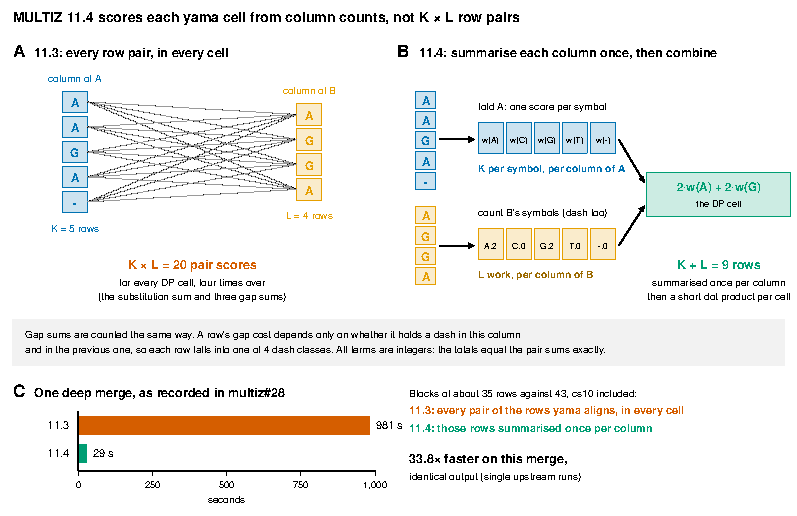
\includegraphics[width=\textwidth]{figure1.pdf}
\caption{\textbf{Column counts turn $K \times L$ work per cell into $K + L$ work per column.} In panel A, release 11.3 scored
a toy column pair of $K = 5$ and $L = 4$ rows by visiting all 20 row pairs, once for the substitution sum and once for
each of three gap sums. In panel B, release 11.4 folds the column of $A$ into one score per symbol and counts the symbols of
$B$'s column, each once per column. The cell is their dot product, here $2 w(\mathrm{A}) + 2 w(\mathrm{G})$. Gap sums
are counted by four dash classes. Blue marks $A$, orange $B$, green the 11.4 cell and vermilion the 11.3 row-pair
work. Panels A and B are a toy example, not data. Panel C is the deep merge recorded in \code{multiz\#28}, one run per
release.}
\label{fig:explainer}
\end{figure}

\section{What it measured}
\label{sec:measured}

\paragraph{Synthetic blocks.} To measure the scaling on public, reproducible input, we built 11.3 and 11.4 from
their release tags with identical flags (\code{-O2}) and merged synthetic block pairs with $K = L$ from 2 to 128.
Each pair has 10 blocks of 2,000 reference columns, a shared reference row, species rows with 2 percent substitutions
and 1 percent deletions, and insertion columns placed differently in the two files, so \code{yama} has columns to
align. Times are medians of three runs (Table~\ref{tab:sweep}, Fig.~\ref{fig:sweep}). The 11.3 time rose about four
times for each doubling of $K$, as $K \times L$ predicts, from 0.34\,s at $K = 8$ to 76.7\,s at $K = 128$. The 11.4
time stayed between 0.06 and 0.13\,s up to $K = 32$ and reached 1.22\,s at 128. The speed-up was 5.4-fold at
$K = 8$, 37-fold at 32 and 63-fold at 128. Outputs were identical at all seven depths.

\begin{table}[t]
\centering
\small
\caption{\textbf{Synthetic block pairs, median of three runs per release.} Identical: the two outputs agree after
removing \code{\#} header lines.}
\label{tab:sweep}
\begin{tabular}{rrrrrc}
\toprule
$K = L$ & $K \times L$ & v11.3 (s) & v11.4 (s) & speed-up & identical \\
\midrule
2 & 4 & 0.057 & 0.061 & 0.93 & yes \\
4 & 16 & 0.113 & 0.059 & 1.92 & yes \\
8 & 64 & 0.340 & 0.063 & 5.37 & yes \\
16 & 256 & 1.282 & 0.076 & 16.84 & yes \\
32 & 1{,}024 & 4.842 & 0.129 & 37.45 & yes \\
64 & 4{,}096 & 19.412 & 0.322 & 60.35 & yes \\
128 & 16{,}384 & 76.733 & 1.220 & 62.92 & yes \\
\bottomrule
\end{tabular}
\end{table}

\begin{figure}[t]
\centering
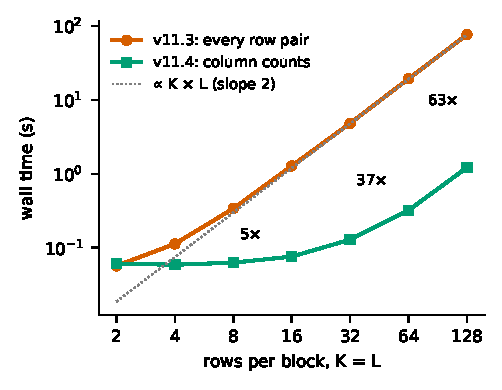
\includegraphics[width=0.55\textwidth]{figure2.pdf}
\caption{\textbf{The 11.3 time follows $K \times L$, and the 11.4 time grows far more slowly.} Wall time of one
\code{multiz} merge of a synthetic block pair against block depth, log-log, median of three runs. Vermilion
circles are v11.3, green squares v11.4, and the dotted line has slope 2 through the last v11.3 point. Labels give
the speed-up. Below $K = 4$ both releases spend their time outside \code{yama}.}
\label{fig:sweep}
\end{figure}

\paragraph{Product, not square.} With $K = L$ the sweep cannot tell $K \times L$ from $K^2$. A grid of unequal depths,
$K$ and $L$ each 4, 16 or 64, separates them (Fig.~\ref{fig:grid}). The 11.3 time depended on the product alone.
At $K \times L = 256$, the $4 \times 64$, $16 \times 16$ and $64 \times 4$ pairs took 1.27, 1.25 and 1.46\,s, and at
1,024 the $16 \times 64$ and $64 \times 16$ pairs took 4.83 and 4.80\,s, against 4.84\,s for $32 \times 32$. All
nine outputs were identical.

\paragraph{Where the time goes now.} The 11.4 time does not stay proportional to $K + L$ at depth. From
$K = L = 64$ to 128 it rose 3.8-fold. A \code{gprof} profile of the $K = L = 128$ merge shows why
(\code{measurements/gprof\_k128.txt}). In 11.3, \code{yama} took 76.7\,s of 77.8 and \code{mafScoreRange} 1.1\,s.
In 11.4, \code{yama} took 0.06\,s, about a thousand times less, while \code{mafScoreRange} still took 1.1\,s, now
94 percent of the run. \code{mafScoreRange} scores each merged block by summing over all pairs of its
$K + L - 1$ rows, so it grows with the square of the total depth. That caps the speed-up near 60-fold in this sweep.
The same counting would apply to it, which makes it the next target.

\begin{figure}[t]
\centering
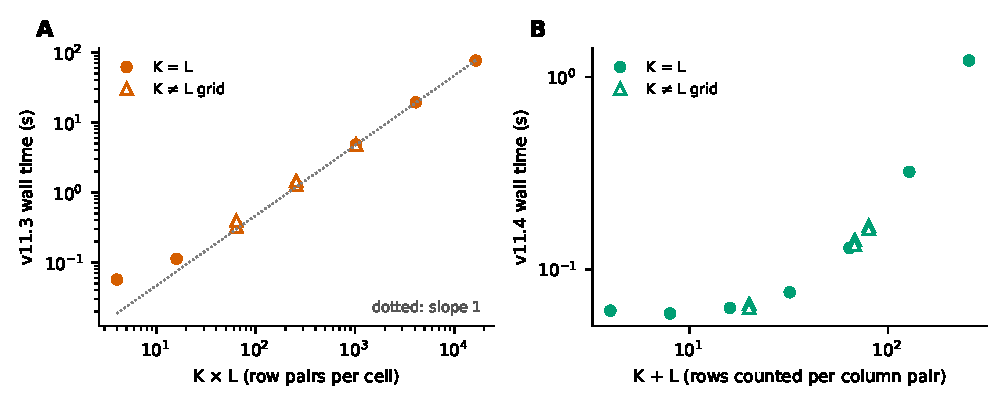
\includegraphics[width=\textwidth]{figure3.pdf}
\caption{\textbf{The 11.3 time depends on $K \times L$, whatever the shape of the pair.} Panel A plots the v11.3 wall
time against $K \times L$ and panel B the v11.4 time against $K + L$, both log-log. Filled circles are the $K = L$
sweep, open triangles the grid with $K \neq L$ (each of 4, 16 and 64). The dotted line in A has slope 1. Medians of
three runs, all outputs identical. In B the time is flat at about 0.06\,s for small depths, where little time is
spent aligning, and grows faster than $K + L$ at large depths, where \code{mafScoreRange} dominates.}
\label{fig:grid}
\end{figure}

\paragraph{Real merges.} The pull request that introduced the change records three more
measurements~\cite{multiz28}. The deep merge above took 981\,s with the 11.3 release build and 29\,s with 11.4, and
its output and both files of unused blocks were identical apart from the header line. A whole 216-genome roast of
one 4.4\,Mb \emph{Cannabis} piece took a median 14,085\,s with 11.3 and 2,873\,s with 11.4 (4.9-fold, 4.5- to
5.2-fold across single-run pairings), three interleaved runs per release on one host, all six outputs identical
apart from \code{\#} lines. UCSC's hg38 \code{multiz5way} recipe still reproduced the published alignment, 7 of 7
sequences.

\paragraph{Why a whole run gains less.} A roast merges along the whole guide tree, and the merges low in the tree are
shallow. At shallow depth \code{yama} is not the bottleneck: in the sweep, 11.3 and 11.4 differ by under 2-fold
below $K = 8$. Block scoring, projection and file handling also take time that this change does not touch. So the gain on a whole
run depends on how much of it is spent in deep merges, which is why one deep merge gained 33.8-fold and a whole
piece 4.9-fold.

\section{Prior work}

Neither half of the change is new.

Scoring a column from symbol counts is a profile. Gribskov, McLachlan and Eisenberg defined the profile score of
symbol $a$ at position $p$ as $M(p,a) = \sum_b W(p,b)\, Y(a,b)$, with $Y$ the substitution matrix and the simple
weight $W(p,b)$ the count of residue $b$ in that column divided by the number of sequences~\cite{gribskov1987}. The
fold $w_A$ above is the same sum without the division.

Counting gap states per column to escape the $K \times L$ loop is Gotoh's. Gotoh gave exact sum-of-pairs algorithms
for aligning two groups of sequences~\cite{gotoh1993}, and then removed their cost in proportion to the product of
the group sizes. In his words, profile vectors could already reduce the work, but ``there has been no way to
evaluate the accurate gap-opening costs with computation steps less than $O(M \times N)$''~\cite{gotoh1994}. He did
it with gap-state variables computed once per column and combined during the recursion, and reported speed-ups of
about 10-fold when $M \times N \approx 200$ and over 100-fold when $M \times N > 2{,}500$. His gap states track runs
of any length, because his objective counts gaps exactly. \code{yama}'s quasi-natural costs look back one column,
so the states reduce to four classes.

Exact gap counting is what makes the general problem hard. With linear gap costs counted exactly, aligning two
alignments under the sum-of-pairs objective is NP-complete~\cite{kececioglu2004}, and Kececioglu and Zhang had
earlier relaxed it with optimistic and pessimistic gap counts~\cite{kececioglu1998}. Release 11.4 does not touch that
problem. It computes \code{yama}'s existing objective, quasi-natural gaps included, exactly and faster.

A search on 5 November 2026 (\code{measurements/prior\_art\_search.md}) found no publication that applies this
reduction to MULTIZ or the threaded blockset aligner.

\section{Limits}

\begin{itemize}
\item The sweep's blocks are synthetic: uniform random sequence, fixed mutation rates, one seed, equal depths
  $K = L$. They show how the cost scales with depth, not how a real alignment behaves.
\item The sweep ran on a 32-vCPU host while unrelated single-threaded alignment jobs were running (load average
  about 4.8). Each \code{multiz} run is single-threaded, and the two releases ran back to back for each size.
\item The profiles are \code{gprof} samples at 0.01\,s, so the 0.06\,s for \code{yama} in 11.4 is coarse. It
  supports ``about a thousandfold'', not a precise ratio.
\item The deep-merge and whole-piece timings are taken from the pull request and were not rerun for this note. The
  deep merge is one run per release.
\item Output identity was checked on the seven synthetic pairs, the deep merge, the whole piece and the hg38 5-way
  recipe. It is an empirical check of the exactness argument, not a proof.
\end{itemize}

\section*{Methods and availability}

\code{probe/build\_multiz.sh} clones \code{multiz} at tags \code{v11.3} (commit \code{645ab55}) and \code{v11.4}
(\code{6bfe6a4}) and builds both with \code{-O2 -Wall -Wextra} (gcc 15.2.0). \code{probe/make\_blocks.py} writes the
synthetic pairs (seed 1), and \code{probe/run\_sweep.py} times them and compares outputs, writing
\code{measurements/sweep.csv} ($K = L$) and \code{measurements/grid.csv} (\code{-{}-sizes 4x4,4x16,\ldots,64x64}).
\code{probe/profile\_k128.sh} builds both releases with \code{-pg} and writes \code{measurements/gprof\_k128.txt}. The host is recorded in \code{measurements/sweep\_env.txt}. Figures are made by
\code{paper/make\_figure1.py}, \code{paper/make\_figure2.py} and \code{paper/make\_figure3.py}. MULTIZ is at \url{https://github.com/multiz/multiz}.
Text, figures and code are CC0 1.0.

\section*{Acknowledgements}

Minmei Hou suggested describing the change as reducing $K \times L$ work to $K + L$.

\begin{thebibliography}{9}

\bibitem{altschul1989} S.~F. Altschul. Gap costs for multiple sequence alignment. \emph{Journal of Theoretical
Biology} 138:297--309, 1989. doi:10.1016/S0022-5193(89)80196-1.

\bibitem{blanchette2004} M.~Blanchette, W.~J. Kent, C.~Riemer, et~al. Aligning multiple genomic sequences with the
threaded blockset aligner. \emph{Genome Research} 14:708--715, 2004. doi:10.1101/gr.1933104.

\bibitem{chao1994} K.-M. Chao, R.~C. Hardison and W.~Miller. Recent developments in linear-space alignment
methods: a survey. \emph{Journal of Computational Biology} 1:271--291, 1994. doi:10.1089/cmb.1994.1.271.

\bibitem{gotoh1993} O.~Gotoh. Optimal alignment between groups of sequences and its application to multiple sequence
alignment. \emph{Computer Applications in the Biosciences} 9:361--370, 1993. doi:10.1093/bioinformatics/9.3.361.

\bibitem{gotoh1994} O.~Gotoh. Further improvement in methods of group-to-group sequence alignment with generalized
profile operations. \emph{Computer Applications in the Biosciences} 10:379--387, 1994.
doi:10.1093/bioinformatics/10.4.379.

\bibitem{gribskov1987} M.~Gribskov, A.~D. McLachlan and D.~Eisenberg. Profile analysis: detection of distantly
related proteins. \emph{Proceedings of the National Academy of Sciences USA} 84:4355--4358, 1987.
doi:10.1073/pnas.84.13.4355.

\bibitem{kececioglu1998} J.~Kececioglu and W.~Zhang. Aligning alignments. In \emph{Combinatorial Pattern Matching
(CPM 1998)}, Lecture Notes in Computer Science, 189--208, 1998. doi:10.1007/BFb0030790.

\bibitem{kececioglu2004} J.~Kececioglu and D.~Starrett. Aligning alignments exactly. In \emph{Proceedings of the
Eighth Annual International Conference on Research in Computational Molecular Biology (RECOMB 2004)}, 85--96, 2004.
doi:10.1145/974614.974626.

\bibitem{multiz28} multiz/multiz pull request 28, ``yama: build each cell's sums from column counts, not row pairs''
(2026). \url{https://github.com/multiz/multiz/pull/28}.

\end{thebibliography}
\end{document}
